\documentclass[12pt, a4paper]{scrartcl}
\usepackage[utf8]{inputenc}

\usepackage{graphicx}
\usepackage{fancyhdr}
\usepackage{url}
\usepackage{listings}
\usepackage{booktabs}
\usepackage{palatino,avant}
\usepackage[ngerman]{babel}
\usepackage[pdftex,bookmarks=true,bookmarksnumbered=true,bookmarksopen=true,colorlinks=true,filecolor=black,
                linkcolor=red,urlcolor=blue,plainpages=false,pdfpagelabels,citecolor=black,
                pdftitle={VSY-Dokumentation},pdfauthor={Michael Stapelberg}]{hyperref}
\begin{document}
\pagestyle{fancy}
\chead{VSY}
\lhead{Bullshit-Bingo}
% New paragraph
\newcommand{\np}{\bigskip\noindent}

% No indention at new paragraphs
\setlength{\parindent}{0pt}

\lstset{%
	basicstyle=\small\ttfamily,%
	showstringspaces=false,%
	frame=single,%
}


\author{\\
von\\
Faraz Ahmed\\
Felix Bruckner\\
Dennis Cisowski\\
Michael Stapelberg\\
Thorsten Töpper\\
~}
\title{Dokumentation Bullshit-Bingo}
\subtitle{Vorlesung Verteilte Systeme im SS2011}

\maketitle
\clearpage

\tableofcontents

\clearpage
\section{Architektur}

Als Architektur haben wir uns für ein Client/Server-Modell entschieden, da es
deutlich einfacher zu implementieren ist als ein Peer-to-Peer-Netz. Bei
letzterem gibt es das Problem des Nachrichtentransports: Entweder müssen alle
Peers sich mit allen anderen verbinden um in der Lage zu sein, Nachrichten an
alle zu senden (Full-Mesh) oder man braucht eine Form der
Nachrichtenweitergabe. Bei einem Client/Server-Modell entfällt diese
Problematik. Weiterhin ist bei dieser Architektur der Bezug zur tatsächlichen
Praxis höher, bei der Peer-to-Peer-Netze selten eingesetzt werden\footnote{Eine
bekannte Ausnahme stellt World of Warcraft mit dem BitTorrent-gestützten Update
Downloader dar}.

\subsection{Basis-Protokoll: HTTP}

Das grundlegende Protokoll, welches wir verwenden, ist HTTP. In der Praxis
verwendet man aus mehreren Gründen gerne HTTP:
\begin{itemize}
	\item Das Protokoll verwendet ASCII (statt Binärdaten) in einem
	einfachen, für Menschen lesbaren, Format.

	\item Implementationen sind in jeder ernstzunehmenden
	Programmiersprache ver\-füg\-bar und in der Regel weitreichend getestet.

	\item HTTP ist in den meisten Firewalls freigeschaltet, weil das World
	Wide Web eine so weit verbreitet Technologie des Internets darstellt.

	\item Zusätzliche Software wie Load-Balancer, Proxies, etc. sind für
	HTTP bereits verfügbar (auch als direkt in Hardware implementierte und
	somit sehr performante Varianten).
\end{itemize}

\subsection{Serialisierung: JSON}

Zum Serialisieren von Daten verwenden wir für beide Seiten (also für Requests
vom Client an den Server und für Antworten des Servers zum Client) die
JavaScript Object Notation (JSON).
\np

Der geringe Umfang von JSON (Arrays, Maps/Hashes, Strings, Numbers) macht es
einfach, entsprechende Bibliotheken in allen ernstzunehmenden
Programmiersprachen zu implementieren. Außerdem ist JSON (bei geeigneter
Formatierung) leicht für Menschen lesbar. Im Gegensatz zu XML ist der Overhead
sehr gering.

\subsection{Protokoll}

Mithilfe von HTTP und JSON haben wir eine Protokolldefinition erstellt (siehe
Datei \texttt{PROTOCOL}), welche festhält, welche URLs mit welchen Parametern
aufgerufen werden, was dieser Aufruf bewirkt und mit welcher Antwort man zu
rechnen hat.

\clearpage

\section{Server}

Wir haben den Server in Perl implementiert, da Perl eine moderne Sprache ist,
die es einem ermöglicht, in kurzer Zeit sauber strukturierte und performante
Programme zu schreiben.
\np

Auf folgende Module haben wir aufgebaut:
\begin{description}
	\item[Moose] Moose\footnote{\url{http://www.iinteractive.com/moose/}}
	ist ein modernes Objektsystem für Perl. Vereinfacht die Implementation
	von objekt-orientierten Modulen.

	\item[Tatsumaki] Ein asynchrones und hoch-performantes Web-Framework
	(auf Basis des Web-Stacks Plack und dem Event-basierten AnyEvent).

	Ein anderes, sehr beliebtes Framework, welches wir ebenfalls hätten
	verwenden können, ist
	Dancer\footnote{\url{http://www.perldancer.org/}}.

	\item[JSON::XS] Ein Modul zum Enkodieren/Dekodieren von JSON,
	implementiert in C für hohe Geschwindigkeit.

	\item[Test::More] Ein Modul zum Implementieren von Test-Cases,
	begleitet von exzellenter
	Dokumentation\footnote{\url{http://search.cpan.org/perldoc?Test::Tutorial}}.
\end{description}

\subsection{Test Driven Development}

Wie in der Perl-Welt üblich sind wir nach dem Modell des \textsc{Test Driven
Development} vorgegangen. Das heißt, wir haben zunächst die Testcases
implementiert (siehe Verzeichnis \texttt{t/}) und anschließend die
Implementation so durchgeführt, dass alle Tests erfolgreich ausgeführt werden.
\np

Folgendermaßen sieht einer unserer Tests aus:
\begin{lstlisting}[language=Perl]
my $json = post('CreateGame', { token => $token, size => 3 });
is($json->{success}, JSON::XS::true, 'Game created');
ok(exists $json->{id}, 'game id included in reply');
ok(exists $json->{words}, 'game words included in reply');
ok(exists $json->{name}, 'game name included in reply');
like($json->{name}, qr/^Unbenannt /, 'name starts with "Unbenannt"');
is(@{$json->{words}}, 9, 'nine words for a 3x3 game delivered');
\end{lstlisting}

\clearpage
\section{Qt-Client}

Qt (gesprochen: cute) ist ein GUI-Framework für C++, welches
plattformunabhängig zur Verfügung steht und von Nokia entwickelt wird.

Da Qt-Kenntnisse in der Gruppe bereits vorhanden waren und man zur Abwechslung mal wieder einen Abstieg in die C++-Pointerhölle unternehmen konnte, entschieden wir uns prompt dazu eine solche Variante unseres Clients zu implementieren.
\np

\subsection{Eingesetzte Bibliotheken \& Software}
Da sich C++-Programme nur nativ übersetzen lassen und wir unterschiedlichste 
Betriebssysteme sowohl privat als auch zur Bearbeitung dieser Aufgaben im Einsatz 
haben, setzen wir anstatt der klassischen Makefiles CMake
\footnote{"Cross-Platform Make", \url{http://www.cmake.org/}} als Buildsystem ein.
\np
 
Qt liefert eine Anzahl an nützlichen Bibliotheken von Haus aus mit, demnach
können wir für Netzwerk-Funktionalität einfach die QNetwork-Bibliothek verwenden.
Um JSON-Daten vom Server auszuwerten, müssen wir jedoch auf Drittsoftware
zurückgreifen und benutzen die bewährte QJson\footnote{\url{http://qjson.sourceforge.net/}}-Bibliothek.
\np
\subsection{Architektur}
Die Architektur des Qt-Clients

\subsubsection{Grundidee}
Grob umrissen wird folgendes Kommunikationskonzept eingesetzt:

\begin{itemize}
	\item Clientseitig spezielle JSON-Requestobjekte serialisieren und per POST/GET via http an den Server senden.
	\item Antworten in Rohform in Nutzdaten wandeln und auswerten.
\end{itemize}

Dabei wird stark auf Qt-spezifische Features zurückgegriffen, unter anderem Q\_Properties, die mithilfe des MOC\footnote{Meta Object Compiler} in einfach serialisierbare Klassen übersetzt werden können, sowie das QVariant-Konstrukt als Container für beliebige Nutzdaten.   


\subsubsection{Programm-Architektur}
\begin{center}
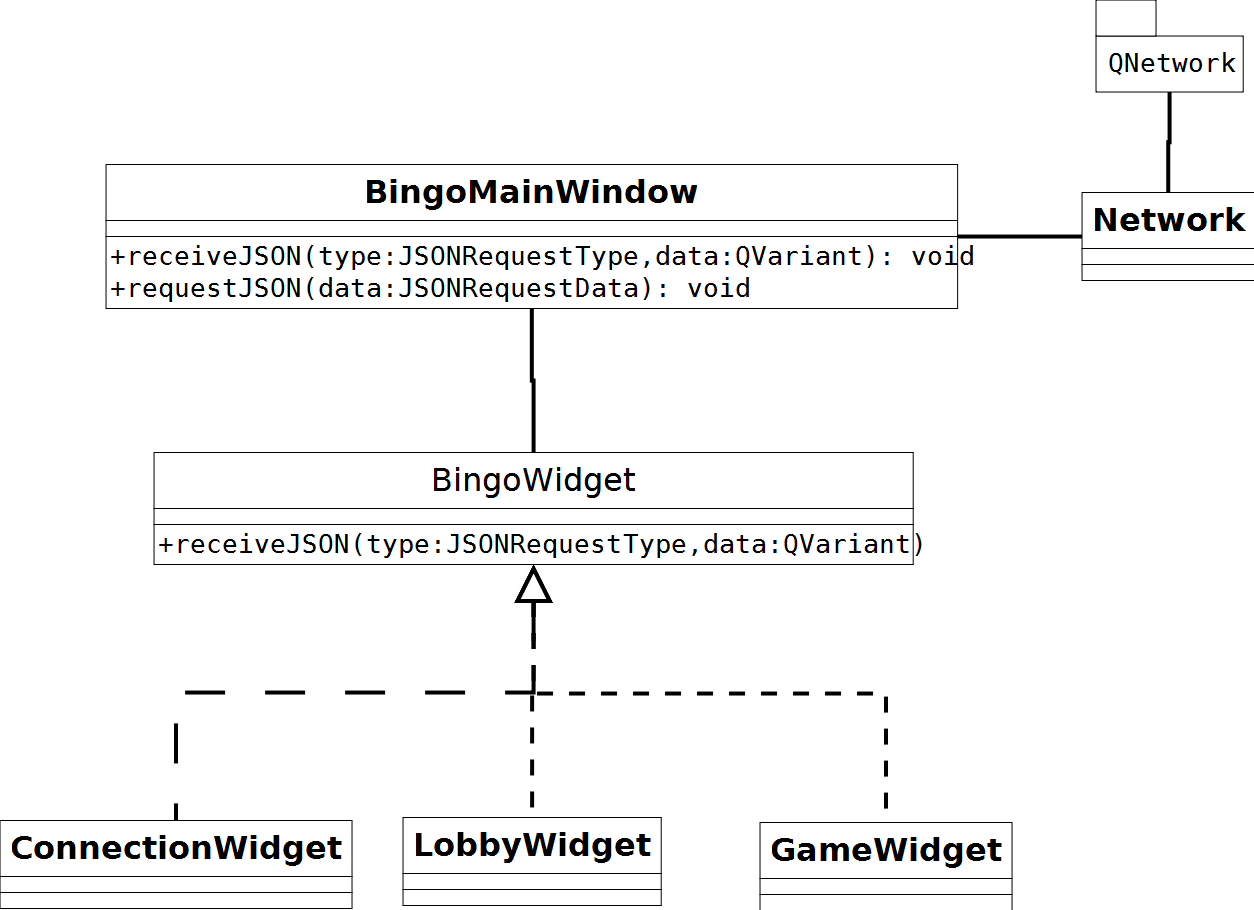
\includegraphics[height=10cm]{qt-klassendiagramm.png}
\end{center}
\np

Das Herzstück bildet das \textbf{BingoMainWindow}\footnote{Erweitert QMainWindow, stell also ein Applikations-Hauptfenster mit Menü, Statusleiste und Fensterdekoration dar.}, durch welches die gesamte Benutzerinteraktion handhabt und den Widgets erlaubt, Netzwerkzugriffe abzusetzen.\np

Des Weiteren wird eine Art Observer-Pattern eingesetzt: Jedes \textbf{Widget} ist automatisch Listener
für Netzwerk-Antworten, welche die Netzwerkkomponente empfängt - das zurzeit aktive (= für den Benutzer sichtbare) erhält die Daten.\np

Die \textbf{Network}-Klasse ist mehr oder minder ein Wrapper einiger QNetwork-Funktionen, um Objekte vom Typ JSONRequest anhand ihrer Properties\footnote{Siehe \url{http://doc.qt.nokia.com/latest/qobject.html\#Q_PROPERTY}} in valides JSON zu serialisieren, daraus eine HTTP-Anfrage zu formen, diese asynchron abzusetzen und mithilfe eines Callbacks die Anwort zu erhalten und weiterzureichen.

\clearpage
\section{Java-Client}

Im Studium an der HS-Mannheim lernt man Java. Den kleinsten gemeinsamen Nenner
in Sachen Programmiersprache auf die Praxis-Probe zu stellen ist daher nur
logisch.
\np

\subsection{Verwendete Bibliotheken}
Zur grafischen Darstellung der Benutzeroberfläche verwenden wir das
\texttt{Swing} Framework, da dies viele Dinge gegenüber dem vorherigen 
\texttt{AWT} Framework vereinfacht.
\np

Zur Serialisierung und Deserialisierung verwenden wir die von JSON.org gebotene
Bibliothek\footnote{\url{https://github.com/douglascrockford/JSON-java}}. Diese
ermöglicht das angenehm einfache Arbeiten mit den Klassen \texttt{JSONObject}
und \texttt{JSONArray}, welche für die direkte Nutzung in unserem Client ausreichen.
\np

Die HTTP Kommunikation wickeln wir mit Hilfe der \texttt{HTTPClient}\footnote{
\url{http://hc.apache.org/}} Bibliothek der Apache Foundation\footnote{
\url{http://www.apache.org}} sehr einfach ab. Zur Kommunikation mussten war nur
die Implementierung zwei Funktionen notewendig, je eine für \texttt{POST} und
\texttt{GET} Requests. Die Funktionen erhalten die bereits serialisierten Daten
als Parameter.
\np

\subsection{Architektur}
Der Client basiert auf einer das \texttt{JFrame} erweiternden Hauptklasse,
welche Objekte der genutzten - auf der \texttt{JPanel} Klasse aufbauenden
- Klassen verwaltet.
\np

Wir verwenden ein Panel für den Login-Prozess, eines als Lobby zur Auswahl
des Spiels, welches ebenfalls die Möglichkeit auf das Panel zur Erstellung
eines eigenen Spiels bereitstellt. Das vierte Panel verwaltet den Spielprozess,
es nutzt einen Thread, welcher in kurzen Zeitabständen prüft, ob ein Spieler
das Spiel gewonnen hat und in etwas größeren Zeitabständen die Liste der
teilnehmenden Spieler aktualisiert.
\np

Der Wechsel zwischen den angezeigten Panels erfolgt über Methodenaufrufe der
Hauptklasse, welche die Eigenschaften dortiger Objekte verändern respektive
die Objekte entfernen.

% TODO: mehr über den java-client

\clearpage

\section{Android-Client}

Da wir bereits Erfahrung mit der Programmierung von Android-Anwendungen haben,
lag es nahe, eine simple Android-GUI zu entwickeln.

\subsection{Implementation}

Damit es ein wenig interessanter wird, haben wir uns entschlossen, diesen in
der recht neuen Programmiersprache Mirah\footnote{\url{http://www.mirah.org/}}
zu implementieren. Mirah ist eine Ruby-ähnliche Sprache auf Basis der
JVM\footnote{Java Virtual Machine}, die im Gegensatz zu anderen JVM-basierten
Sprachen ohne Standardlibrary daherkommt (und somit keine mehrere MB große
Android Packages erzeugt) und keinen Geschwindigkeitsnachteil mit sich bringt
(wie andere Scriptsprachen). Bestechend an Mirah ist die stark an Ruby
angelehnte Syntax, bei der vor allem die andauernden Typdefinitionen wegfallen,
die man in Java hat.
\np

Betrachten wir dazu ein Beispiel aus unserem Code:
\begin{lstlisting}[language=Ruby]
  alert = AlertDialog.Builder.new(self)
  input = EditText.new(self)
  alert.setView input
  alert.setTitle 'Your nickname:'
  alert.setPositiveButton 'Register' do |dialog, which|
    text = input.getText.toString.trim
    Log.d('bullshit', "User entered #{text}")
    RegisterTask.new(activity).execute text
  end
\end{lstlisting}

Das Analogon in Java sähe folgendermaßen aus:
\begin{lstlisting}[language=Java]
  Builder alert = new AlertDialog.Builder(this);
  final EditText input = EditText.new(this);
  alert.setView(input);
  alert.setTitle('Your nickname:');
  alert.setPositiveButton('Register',
    new DialogInterface.OnClickListener() {
      public void onClick(DialogInterface dialog, int which) {
        String text = input.getText().toString().trim();
        Log.d('bullshit', "User entered " + text);
        RegisterTask.new(activity).execute(text);
     }
   });
\end{lstlisting}

Es ist schnell zu erkennen, dass durch die fehlenden Typen, Klammern, Semikola
und insbesondere durch die Blocksyntax im Vergleich zu anonymen Klassen der
Code in Mirah schlanker und einfacher zu lesen ist. Dies ist ein großer Vorteil
beim Programmieren, denn dadurch wird es einfacher, Code zu schreiben (und
insbesondere zu warten), sich in fremden Code einzuarbeiten und Code Reviews
durchzuführen.

\subsection{Techniken}

Der Android-Client verwendet die folgenden wesentlichen Bausteine der
Android-Plattform:

\begin{description}
	\item[AndroidHttpClient] ist eine angepasste Version des Apache
	HTTP-Clients, die sinnvolle Standardeinstellungen für ein mobiles
	Endgerät mitbringt. Die Klasse verwendet knappe Timeouts, teilt
	Instanzen aus einem Pool zu (zwecks Wie\-der\-ver\-wen\-dung) und kann mit
	GZIP-komprimierten Antworten umgehen.

	\item[AsyncTask] stellt eine Aktion dar, die größtenteils im
	Hintergrund ausgeführt wird. Android-Anwendungen laufen standardmäßig
	im sogenannten UI-Thread ab. Die soeben erwähnte
	AndroidHttpClient-Klasse verweigert allerdings aus Effizienzgründen
	ihre Arbeit, wenn man versucht, sie im UI-Thread zu nutzen. Damit soll
	erreicht werden, dass Anwendungen niemals auf Netzwerkzugriff
	blockieren und somit unresponsiv erscheinen.

	Die AsyncTask-Klasse bietet drei Methoden: onPreExecute, doInBackground
	und onPostExecute. Hiervon laufen alle Methoden außer doInBackground im
	UI-Thread ab. In der doInBackground-Methode erledigen wir alle Requests
	zum Server, in den anderen beiden Methoden zeigen wir ggf.
	Fortschrittsdialoge an (beispielsweise beim Betreten des Spiels, nicht
	aber bei den Abfragen nach einem Gewinner).

	\item[Activity, Intent] Eine Activity stellt eine Bildschirmansicht in
	einer Anwendung dar. Wir haben zwei Activities implementiert: Den
	Startbildschirm mit der Übersicht über die derzeit verfügbaren Spiele
	und den Spielbildschirm selbst. Die Frage nach dem Nickname oder das
	Mitteilen eines Gewinners passiert über Dialoge, hierfür verwenden wir
	keine eigene Activity.

	Ein Intent beschreibt eine Absicht, mit der man das Android-System dazu
	veranlasst, zu einer neuen Bildschirmansicht zu wechseln. In unserem
	Fall wechseln wir damit vom Startbildschirm zum eigentlichen Spiel. Den
	Wechsel zurück zum Startbildschirm löst entweder der Benutzer durch den
	Zurück-Button (am Telefon) aus oder das Bestätigen der
	Gewinnermitteilung.
\end{description}

\subsection{Voice Input}

Für das Erreichen aller Coolness-Punkte haben wir Spracheingabe implementiert.
Die Android-API für Spracheingabe zeichnet Ton auf (sie erkennt anhand der
Lautstärke wann der Benutzer anfängt und aufhört zu sprechen) und schickt
diesen an Google-Server. Nachdem diese den Sound ausgewertet haben, kriegt man
eine Liste mit den möglichen Ergebnissen zurück.
\np

Diese Liste vergleichen wir nun mit dem derzeitigen Spielfeld mithilfe der
Levenshtein-Distanz\footnote{\url{http://de.wikipedia.org/wiki/Levenshtein-Distanz}}.
Diese gibt an, wieviele Modifikationen an Wort A erforderlich sind, damit man
Wort B erhält. Sofern die Levenshtein-Distanz kleiner als die Hälfte der
Wortlänge ist, gelten die Wörter bei uns als identisch. Damit erreichen wir
eine verblüffend hohe Trefferrate, zumal die von Google zurückgelieferten
Treffer in der großen Mehrheit der Fälle bereits exakt einem Wort zugeordnet
werden kann.
\np

Die Nutzung der Spracheingabe erfolgt derzeit "`Wort für Wort"'. Das heißt, man
startet die Spracheingabe, spricht sein Wort, das Programm wertet aus, man
spricht das nächste Wort. Auch denkbar ist es, das Telefon einfach im Meeting
mitlaufen zu lassen und ganze Sätze auszuwerten. Dazu müsste man allerdings die
Wörter innerhalb der erkannten Sätze finden, beispielsweise mit dem
Boyer-Moore-Algorithmus\footnote{\url{http://de.wikipedia.org/wiki/Boyer-Moore-Algorithmus}}.

\clearpage
\section{AJAX-Client}

Zwar sind aller guter Dinge drei, aber wenn alle Welt vom Web 2.0 mit
AJAX\--An\-wen\-dung\-en spricht, wollen wir natürlich etwas Praxiserfahrung damit
sammeln und haben kurzerhand unsere vierte Oberfläche als Webanwendung
implementiert.
\np

Zum Einsatz kommt hierbei die JavaScript-Bibliothek
jQuery\footnote{\url{http://www.jquery.com/}}, welche JavaScript in eine kaum
wiederzuerkennende Sprache verwandelt. Sie stellt Hilfsfunktionen für nahezu
alles, was man mit JavaScript treiben könnte (DOM-Manipulation, asynchrone
JSON- oder XMLHTTPRequests, Animationen, etc…).
\np

Weiterhin verwenden wir das
bbq-Plugin\footnote{\url{http://benalman.com/projects/jquery-bbq-plugin/}} um
innerhalb der URL als Fragmente unseren State zu speichern (das Token für den
Spieler sowie die ID des aktuellen Spiels).
\np

Eine typische Funktion sieht beispielsweise so aus:
\begin{lstlisting}
function click_field(token, game, cnt) {
  $.post(
    '/MakeMove',
    JSON.stringify({ token: token, id: game, field: cnt }),
    function(reply) {
      if (reply.success) {
        return;
      }

      alert('Fehler: ' + reply.error);
    }
  );
};
\end{lstlisting}

Mit dem \textdollar{}-Zeichen greift man auf jQuery zu, in diesem Fall rufen
wir die \texttt{post}-Funktion auf, welche einen HTTP POST-Request an die
übergebene URL schickt. Als zweites Argument serialisieren wir die
JavaScript-Datenstruktur nach JSON und als letztes Argument übergeben wir eine
Callback-Funktion, die aufgerufen wird, sobald die Antwort vom Server gelesen
wurde. Da es sich hierbei um den Click-Handler für ein Feld handelt, passiert
bei Erfolg nichts weiter (der Server hat zur Kenntnis genommen, dass das Feld
markiert wurde).
\np

Wir waren erstaunt darüber, in wie wenig Zeilen Code sich ein Client für unser
Bullshit-Bingo in JavaScript mithilfe von jQuery realisieren lässt.

\end{document}
